%!TEX root = ../Main.tex

\chapter[General discussion]{General discussion and final remarks}
\glsresetall
\label{cha:discussion}
%This section wraps up by showing the relationship and importance of a comprehensive approach to data analysis, from the field, genetics, molecular biology and genomics. I will also remark how the technology and the resources have changed in the last 4 years. As at the references used at beginning where superseded during the PhD. 

%Biology is becoming interdisciplinary

%\section{Analysis and tool development for polyploid organisms}

Knowledge from  computer science can be applied to produce software for specific needs, and which can also be useful for the comunity. 
One of the limitations though is that most approaches are developed for diploid systems and are sometimes not compatible with polyploid species, such as wheat. 
Polyploidy adds an extra level of complexity (due to homoeologs) and in the case of wheat the large genome size also hinders certain approaches to genome analyses. Therefore bespoke tools are required to deal with these barriers. 

In this thesis we have taken advantage of technological developments and in genomic resources to generate a series of solutions to several of the problems associated with polyploidy. These methods and approaches are not restricted to wheat, but can be applied and implemented to other polyploid systems.
Diploid species with recent whole genome duplication events (such as \textit{Brassica rapa} and \textit{B. oleracea}; \citealt{Cheng2014}) present similar issues surrounding closely related gene copies and the methods and approaches developed here are likewise applicable.

I have discussed individual the elements of project at the end of each chapter. However, looking forward my interest is to integrate this data into a single scheme. I outline this in Figure \ref{fig:discussion:allTables} and discuss it below. 

\begin{sidewaysfigure}
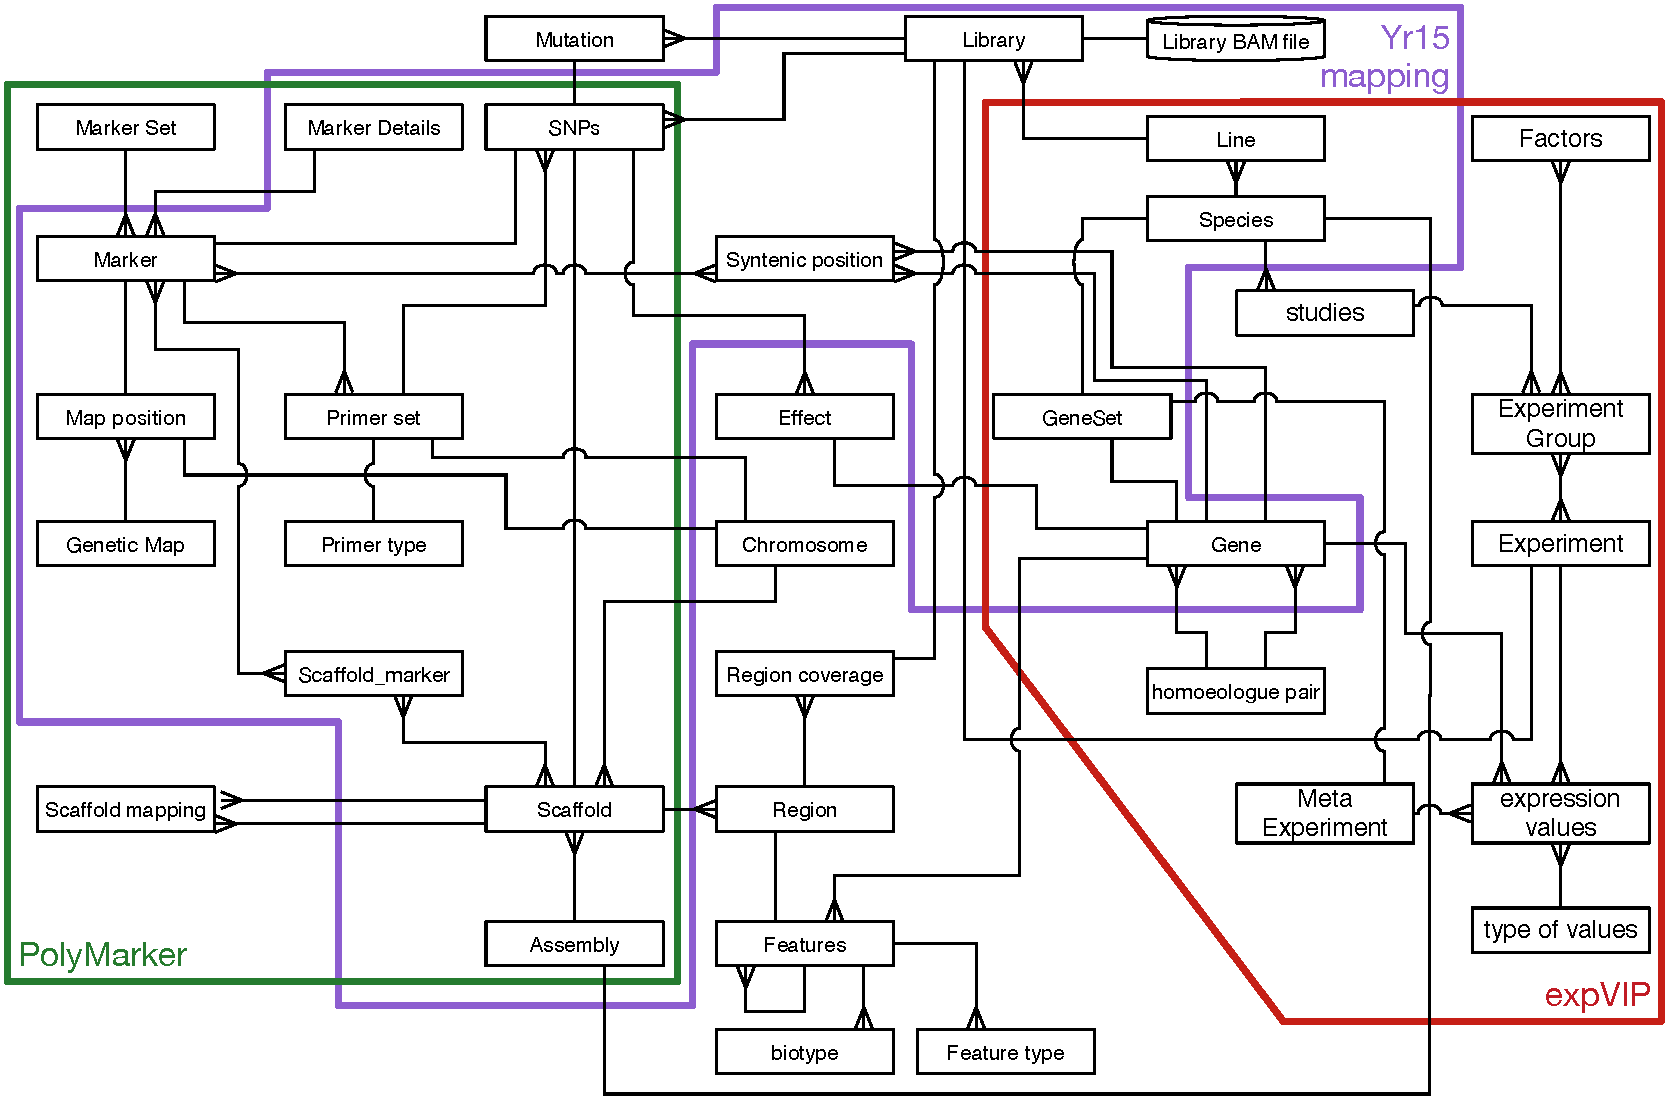
\includegraphics[width=1\textwidth]{Conclusions/Figures/CompleteDatabase.pdf}
\caption[Relational database integrating all the datasets.]{Relational database integrating all the datasets. The boxes represent the tables that contain information related to each chapter.}
\label{fig:discussion:allTables}
\end{sidewaysfigure}

\newpage
\section{Integration of different genetic maps}

Genetic maps are a common starting point to search for a locus linked to a trait, both for breeders and academic researchers. 
For example, in Chapter \ref{yr15} previous genetics maps had already identified the short arm of chromosome 1B as the locus for \acrshort{yr15} \citep{Murphy2009}.
Furthermore, I was able to confirm an enrichment of SNPs linked in the expected region thanks to the mapping of the markers included in the genetic map from \citet{Wang2014} to the \acrshort{css} scaffolds \citep{Mayer2014}. Since my initial analysis, other genetic maps with a higher resolution have been published \citep{Chapman2015, Allen2016,Winfield2016} and these could be further integrated in future analyses. 
The relationship between the tables used in the genetic map is shown in Figure \ref{fig:discussion:geneticMapsTables}

\begin{figure}[b]
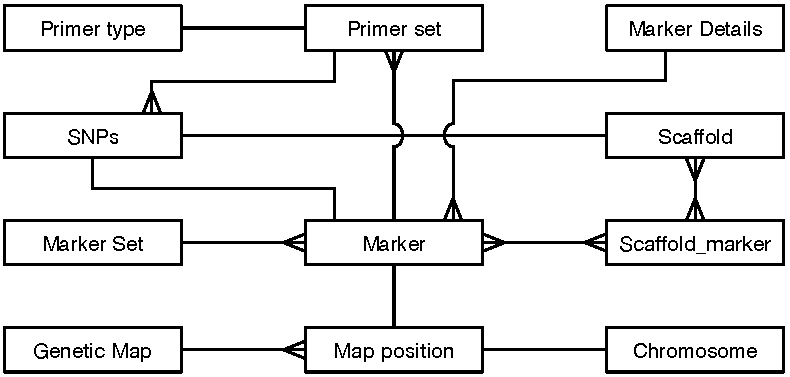
\includegraphics[width=1\textwidth]{Conclusions/Figures/GenetiMapTables.pdf}
\caption{Tables to store information about genetic maps.}
\label{fig:discussion:geneticMapsTables}
\end{figure}

Genetic maps are produced from the genotype of a population with several markers (marker sets). 
Those markers can be developed explicitly for the genetic map or from an already published marker set, usually in the form of an SNP array. 
A database containing several genetic maps should be able to distinguish the origin of the used markers.
However, a genetic map may contain markers from several marker sets as well.
For those reasons, a genetic map is not connected directly to a marker set, but the relationship is maintained through the markers and their position in the genetic map.
For example in \citet{Simmonds2014}, the genetic map across a target locus includes microsatellite, diversity array technology (DArT), CAPS, and SNP array derived KASP markers. 

To be able to use the genetic markers in a genomic context, the sequence of the markers must be mapped to a reference. 
The assembly may be in a single pseudomolecule (such as the new NRGene assembly) molecule or be separated in scaffolds (such as the IWGSC CSS or TGACv1 assemblies). 
If the assembly is fragmented, the  map can be used to anchor the scaffolds to a genetic position. 
If the assembly consist of long scaffolds the genetic map and the positions can be used to find if the lines used for the map have a rearrangement event. 
If a rearrangement is present, the collinearity between the genomic reference and the genetic map is not conserved. 
Having the markers and scaffolds in the database simplifies this kind of analysis, as all the needed data is readily available. 
This will prove important as new genome references become available for a diverse set of wheat varieties as well as high density maps for large mapping populations. 
For example, \gls{ei} are currently re-sequencing Avalon and Cadenza, two important lines in many UK variety pedigrees. 
A large \gls{dh} population from these lines is available and several high density genetic maps have been made from different \gls{snp} arrays \citep{Winfield2016,Allen2016}. 
It will be fascinating to see how the integration of these high density maps and the long range scaffolds produced by the \gls{ei} genomic assemblies will help elucidate local rearrangements which are proposed in this population \citep{Allen2016}.

Furthermore, PolyMarker (Chapter \ref{cha:polymarker}) has been used to design KASP assays for most of the primers in the 90k \citep{Wang2014} and 820k \citet{Winfield2016} SNP arrays. 
The primers for the assays can be integrated in the database. 
This allow a use case were known flanking markers are queried and the database can return a list of possible markers with the primers already designed to be validated on a mapping population. 
This is now routinely done in many labs based on personal communications. 
The general approach has been used in \citet{Simmonds2014} who genotyped NILs with the SNP assays. 
After identifying polymorphic markers these had to be manually converted into KASP assays; the delay in designing primers in this study inspired in part the development of PolyMarker. 
Similarly, many labs routinely use RNA-Seq for SNP discovery and spend several weeks or months in primer design \citep{Shatalina2013}. 
Discussions with this group and others also supported the need to rapidly convert \textit{in silico} SNP data into functional individual SNP assays. 
PolyMarker has largely succeeded in removing this important bottleneck. 

\section{Integration of different genome references. }

The efforts to produce a wheat reference genome had been focused on the \gls{cs} landrace. 
\acrshort{cs} is only cultivated as a research line, as it is susceptible to several pathogens and its yield is inferior to modern varieties.  
The reason for \acrshort{cs} to be the selected cultivar to be sequenced as reference is historic: it has long been a variety  for research.
\acrshort{cs} was originally chosen because it was able to cross with rye. 
It has also been used to produce lines with chromosomic aberrations, useful to find if any particular chromosome is responsible for certain traits \citep{Sears1985}. 
Figure \ref{fig:discussion:assemblyTables} includes the tables used to store assemblies, the relationships between them and their annotation. 

\begin{figure}
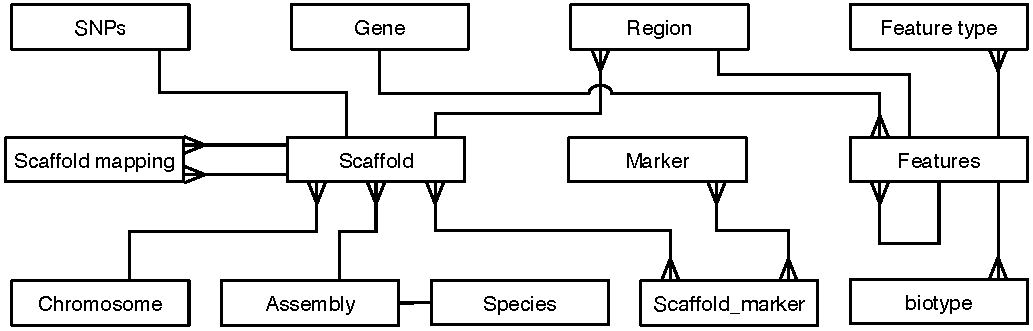
\includegraphics[width=1\textwidth]{Conclusions/Figures/assemblyTables.pdf}
\caption{Tables to store information about genome assemblies and their annotation.}
\label{fig:discussion:assemblyTables}
\end{figure}

New assemblies are required to address the shortcomings of the use of \acrshort{cs} as a genome reference and to include the diversity from other lines \citep{Allen2016,Winfield2016}. 
The assemblies may include their own annotation, and that should be reflected in the database too. 

As of september 2016 there are four sets of genomic sequence used by the wheat community:
\begin{enumerate}
	\item  A 454 whole genome shotgun sequence that is unassembled, and each read is treated as a scaffold \citep{Brenchley2012}.
	\item The genome assembly and annotation from the \gls{css} done by the \acrshort{iwgsc} \citep{Mayer2014}.
	\item A whole genome shotgun sequence from a syntetic wheat, without a corresponding annotation \citep{Chapman2015}.
	\item The whole genome shotgun sequencing and annotation from \acrshort{cs} (TGACv1; \citealt{Clark2016}).
\end{enumerate}

All those references can be aligned to each other to find corresponding regions. 
The corresponding regions can be stored in the scaffold mapping table. 
Furthermore, the scaffolds can be mapped to related species, such as \textit{Brachypodium distachyon}, \textit{Oryza sativa}, \textit{Sorghum bicolor}, and \textit{Hordeum vulgare} to find syntenic blocks. 

Each genome assembly is usually annotated with their genes and other features. 
To include the annotation, each scaffold can contain several features. 
As some features consist on sub-features, like genes conformed by several exons, a recursive relationship is included in the features tables. 
With the support of the scaffold mapping, the different annotations can be projected on different references. 
Gene models, like the ones described in \citep{Krasileva2013}, and  genetic markers can be aligned to any of the reference genomes.

With all those relationships available, the \textit{In silico} mapping in Chapter \ref{yr15} could be produced on several references at once. 
Also, the relationship between different gene models could be simplified, as the corresponding features will share coordinates.
Likewise, the co-expression of genes located in the same region is an useful feature for expVIP (Chapter \ref{cha:exp}). 

\pagebreak
\section{Integration of expression data and beyond}

A database to integrate expression studies was developed for expVIP (Chapter \ref{cha:exp}). 
I designed the database to be as extensible as possible, already with the idea of having an integrated database for different types of resources for wheat. 
To better unify expVIP with the rest of the database, the experiments can be assigned to a particular library. 
In that way, when the RNA-Seq experiment is used for SNP calling, a relationship for it will be available. 
A more comprehensive discussion of the tables in Figure \ref{fig:discussion:expressionTables} is found in Chapter \ref{cha:exp}. 

\begin{figure}[b]
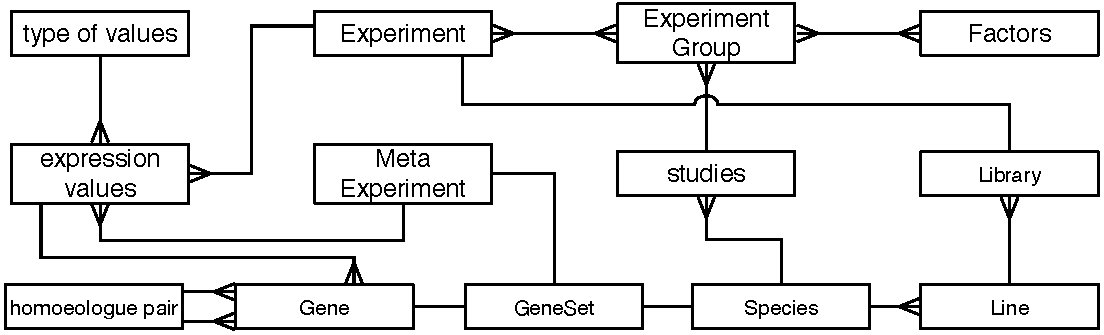
\includegraphics[width=1\textwidth]{Conclusions/Figures/ExpressionTables.pdf}
\caption{Tables to store information about gene expression.}
\label{fig:discussion:expressionTables}
\end{figure}

On Chapter \ref{yr15}, I described how RNA-Seq can be used as a reduced representation method to call for SNPs. 
However, RNA-Seq is primarily used to analyse differential expression, which can be used to find candidate genes involved in a trait.
Other studies have shown that it is possible to do differential expression and SNP calling to improve the candidate genes linked to a trait \citep{Lopez-Maestre2016}.
On the current design of the database it is possible to integrate both types of analyses (Figure \ref{fig:discussion:sequencingExperimentsTables}). 
Because the database is able to integrate previously published studies from different source, it is possible to link the expression to variations previously explored. 

The effect of the SNPs can be predicted with tools like snpEFF \citep{Cingolani2012} or Ensembl VEP \citep{Mclaren2016}. 
I have implemented this part of the database for the \url{http://www.wheat-tilling.com} website, which contains all the mutations, their effects and primers (see Section \ref{sub:poly:muts}) described in \citet{Krasileva2016}. 
Currently the database in the tilling website doesn't include any information regarding the expression. 
Hence, to see if a mutation is in a gene differentially expressed requires a separate visit to \url{www.wheat-expression.com} (Chapter \ref{cha:exp}). 
If the two databases were merged as proposed, it would be possible to have a query to find all the SNPs in genes that are differentially express under certain conditions.
Moreover, this integration would allow users to query for specific mutations which result in truncations in all differentially expressed genes in a given chromosome interval.  

\begin{figure}[b]
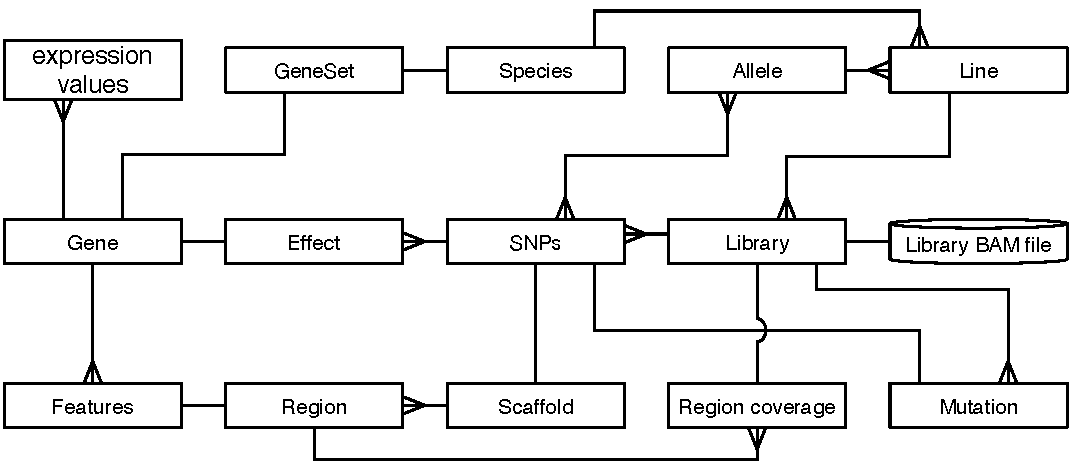
\includegraphics[width=1\textwidth]{Conclusions/Figures/IntegratingExperiments.pdf}
\caption{Relationship of different types .}
\label{fig:discussion:sequencingExperimentsTables}
\end{figure}

To increase the available information, the SNPs and the corresponding alleles for lines with a known genotype  can be added to the database. 
Several varieties had been genotyped with the 820k \citep{Winfield2016} and 90k \citep{Wang2014} SNP arrays, as well as with exome capture methods \citep{Jordan2015}.
Despite being publicly available in CerealsDB, the size of the datasets require specialized bioinformatic knowledge, as regular spreadsheet software is unable to load all the information and stay responsive. 
For that reason, a database to query this datasets would be valuable by itself. 
However, integrating the marker information on the general database can be useful to validate if SNPs called for a studied line are consistent with the expected genotype. 
This kind of validation of the variety of the sample has been done with custom scripts in \citep{Hubbard2015}.
In addition the integration of SNP data across the more contiguous physical sequence now available allows long-range haplotypes to be established. 

Finally, the coverage of certain regions can be stored as counts for the expression analysis, or to analyse the copy-number variation. 
On the same mutant population I have developed an algorithm to detect homozygous deletions from exome capture. 
Since the sequencing is incomplete, finding the exact location where a long deletion starts is difficult. 
However, the relative coverage of the exon can be used as a proxy for the deletion. 
We have proved that for homozygous deletions this approach works (PolyInDel; Section \ref{poly:dels}; \citealt{Krasileva2016}). 
In the future, I would like to extend the algorithm to detect copy number variations. 
Storing the coverage at the exon level in the database, along with the annotation of the deletions, provide another set of candidate genes if the phenotype of a line is known. 

Overall, having a single database with different types of genomic and genetic data, alongside with a reliable annotation can simplify functional genomics. 

%\pagebreak
\section{Integration of sequencing experiments and genetic maps}
%\unsure{Im not sure if I'm repeating the first bit of the discussion, but I think it rounds the idea that everything is related. }
Genomic data by itself is a valuable resource that can help to find SNP markers, differential expression under different condition and structural variation of the genome. 
However, it is not the only available tool for crop scientist and breeders to improve wheat. 
Genetic maps and their associated markers had been used to identify locus linked to traits and for selective breeding, as described in Chapter \ref{yr15}. 

Another source of candidate genes is synteny with relative species \citep{Moore1995}.  
Both \textit{Brachypodium distachyon} and \textit{Hordeum vulgare} can be used as models for wheat as they are closely related diploid organisms with a small genome size (\textit{Brachypodium}) or a more advanced genome sequence (barley; full genome sequence submitted a few weeks ago). 
In the case of barley, the seven chromosomes are mostly collinear \citep{Rustenholz2010} with each of the wheat genomes (A, B and D). 
To take advantage of this relationship, the wheat genetic maps can be linked to genes in more than one species (Figure \ref{fig:discussion:MapVsExpVsSNPvsSyntheni}).
%\unsure{I think something like this has been done in the lab, but can't remember which project.} 
In personal communication with other members of the Uauy group I became aware that it is possible to test the effect of a candidate gene on a related diploid species, where the effect of a change in a single gene can not be hidden by homoeologues genes, as happens in wheat. 

\begin{figure}[h!]
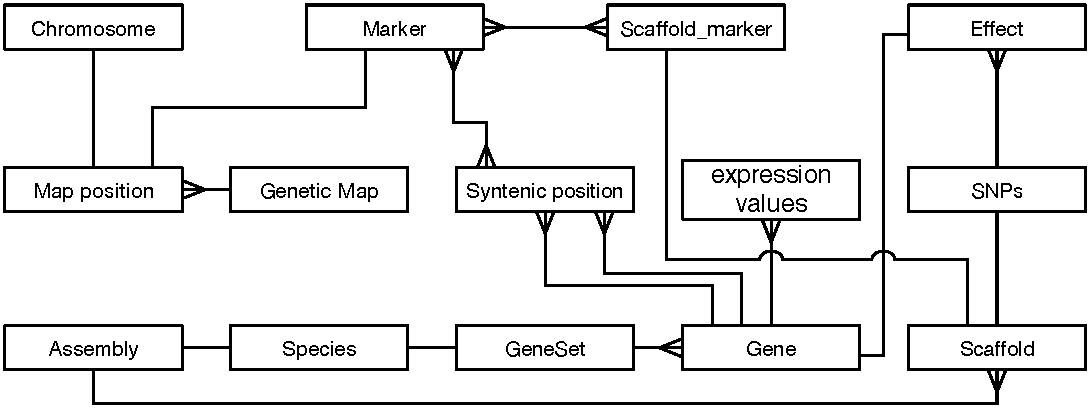
\includegraphics[width=1\textwidth]{Conclusions/Figures/MspVsExpVsSNPvsSyntheni.pdf}
\caption{Tables to store information about gene expression, SNPs and their effects, assemblies and, genetic maps. }
\label{fig:discussion:MapVsExpVsSNPvsSyntheni}
\end{figure}

With a candidate gene tested in a related species, the syntenic relationships can be added as supporting evidence for results coming from different datasets. 
For example, if a gene of unknown function is found to contain a SNP which leads to a premature termination codon, it can be compared to the corresponding gene in barley, which may have a known function.  
Since the gene is mapped to a scaffold, and the scaffold is located in a genetic map, it is possible to validate if there are any QTLs for the same function observed in barley. 
This can be logically extended to better characterised species like rice and can be updated with new information on genes as this becomes available. 


\section{Integration with other services}

Currently, the publicly available wheat resources are scattered as supplemental materials on their corresponding publication or available as \textit{ad hoc} systems focused on a particular field.
For example Ensembl has two different views for every organism: from the genomic point of view and from the expression data. 
The Collaborative Open Plant Omics (COPO; \citealt{Davey2015}) is trying to integrate different sources and types of data by connecting the data providers. 
This approach requires the cooperation of the service providers, which have their own view of what is important. 
I believe that in order to effectively integrate the resources it is necessary to understand how the users are likely to interact with the data.

In order to increase the exposure of PolyMarker (Chatper \ref{cha:polymarker}) and \gls{expvip} (Chapter \ref{cha:exp}), an integration with other online resources is necessary. 
So far, expVIP links to Ensembl to get the details of a displayed gene. 
However, there is no link back from a gene in Ensembl to expVIP. 
To address this it should be possible to contact Ensembl to link back, but it may require a custom interface between both sites. 
This requires an active effort from all the service providers. 
Initiatives like COPO try to reduce the friction between data providers, by providing a common language between sites. 
In the future, the proposed database and the webservices described earlier should implement an interface to communicate with other databases. 

%\pagebreak
\section{Final remarks}

I started my PhD with a strong computational background, but with a limited knowledge of wheat genetics and breeding.
When I was looking for a PhD I wanted an interdisciplinary supervisory team, with a member with bioinformatic background on one side, an one with a strong knowledge of biology. 
Since I had previous experience with processing sequencing data, the project led by Mario Caccamo and Cristobal Uauy on using sequencing to improve wheat caught my attention.

On the first year of my PhD I did what at the time seemed as regular bioinformatic analysis: aligning sequences and calling for \glspl{snp}. 
However, as the project of the mapping of \textit{Yr15} progressed I found out more about genetics and how it is impossible to interpret sequencing data without understanding the context surrounding the experiment (Chapter \ref{yr15}). 
As I got more involved in the genetic mapping project I took the opportunity to go and work in the lab to complement my bioinformatic abilities. 
I was able to run the KASP assays I had designed and develop the genetic maps for my publication. 
I also confirmed that the wet lab is not my vocation, but I can better appreciate the work behind it. 
Also, I found out that the level of uncertainty when doing the experiments in the wet lab is higher than doing the computational analysis and the importance of generating high-quality data interpretation before initiating wet-lab work.

While working on the wet lab I figured out that some of the common analysis can be automated, like the primer design. 
When I faced the prospect of designing manually 50 primers to validate the SNPs and generate a genetic map for \textit{Yr15} I thought that it is the kind of job that computers can do faster with less mistakes. 
This led me to take the initiative to make an automated pipeline to design primers in polyploid organisms (PolyMarker, Chapter \ref{cha:polymarker}).
To properly design PolyMarker I had to understand the relationship between the three genomes of wheat and the caveats of working with the \acrshort{css} assembly, which I helped to assemble before starting my PhD. 
That also changed my vision of bioinformatics. 
I figured out that it is not necessary to have the perfect reference, or the most sound method, if the resource you are producing is not accessible to the target community. 

It was around that time that I noticed that the number of available resources for wheat was growing faster than the community could learn how to use them effectively. 
For example, the development of a massive number of markers can be used to produce high resolution genetic maps, with the right population. 
However, the size of the tables represent a problem to excel, one of the common tools used to organise tables. 
Having a computational background I thought that the kind of queries that could be done with those files could be implemented as a relational database. 
At that point the CSS scaffolds were adopted by the community, despite being relatively short, they enabled analyses that were impossible before. 
I figured out that the high resolution maps could be used to give some order to the scaffolds, and part of me wanted to make an improved version of the scaffolding tool I worked on for the pig genome \citep{Groenen2012a}.
However, the assembly didn't have enough resolution to produce a proper pseudo-molecule and other efforts were being carried out to improve the assembly.

Nevertheless, the idea of integrating different types of data matured enough as to start writing a prototype of the database. 
When discussing with the group how to make available the public RNA-Seq samples deposited by the community I believed that I could leverage on part of my design to power an expression browser. 
Originally, we thought on looking for other open source expression browsers, but none of them had the flexibility required to work on polyploids and they were designed with model organisms in mind, with stable resources and conventions followed by the community. 
So I decided to write the the expression browser that eventually became expVIP (Chapter \ref{cha:exp}). 
For the visualisation I leveraged on my previous experience developing BioJS components, as I worked on a component to visualize BAM files in the browser, under the Google Summer of Code in 2014. 

During the last year I extended the database design and implementation, as we required to display the data from the tilling population described in \citet{Krasileva2016}. 
As the data grew in size and complexity, a single table containing all the mutations with their corresponding effects and primers was not enough. 
Since I already had been developing a prototype of the database to simplify my own analysis when combining data sources, I thought it would be possible to leverage on that code. 
However, the tables that would be useful for the database were different to the tables I had developed already. 
At the end, the combination of the expression and tilling databases, combined with my initial prototype conform the relationships described in the final discussion (this chapter). 

After the four years of my PhD I became convinced that in order to produce bioinformatic software that is powerful and usable it is a requirement to understand both the biological processes to solve as well as the computational methods and software development practices to be be implemented.
